% =====================================
% FIGURAS CAPITULO  TRANSFORMERS
% =====================================

% =====================================
% FIGURA REPRESENTACIÓN MATRIZ X ENTRADA
% =====================================
\newcommand{\MatrizX}{
    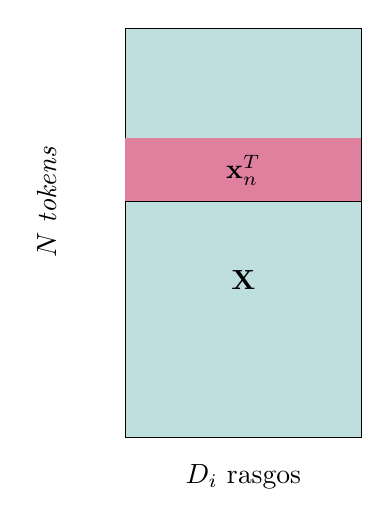
\begin{tikzpicture}[scale=1]

        % Rectángulo grande X
        \fill[teal!50, opacity=0.5] (0,0) rectangle (3,5.2);
        \draw (0,0) rectangle (3,5.2);
        \node at (1.5,2) {$\mathbf{X}$};

        %token x_n
        \draw (0,3) rectangle (3,3.8);
        \fill[purple!50, opacity = 1] (0,3) rectangle (3,3.8);
        \node at (1.5,3.4) {$\mathbf{x}_n^{T}$};

        \node[rotate=90] at (-1,3) {$N$ \textit{tokens}};
        \node at (1.5,-0.5) {$D_i$ rasgos};


    \end{tikzpicture}
}


% =====================================
% FIGURA FLUJO DE DATOS ATENCION MULTIPLE
% =====================================

\newcommand{\FlujoAtencionMultiple}{
    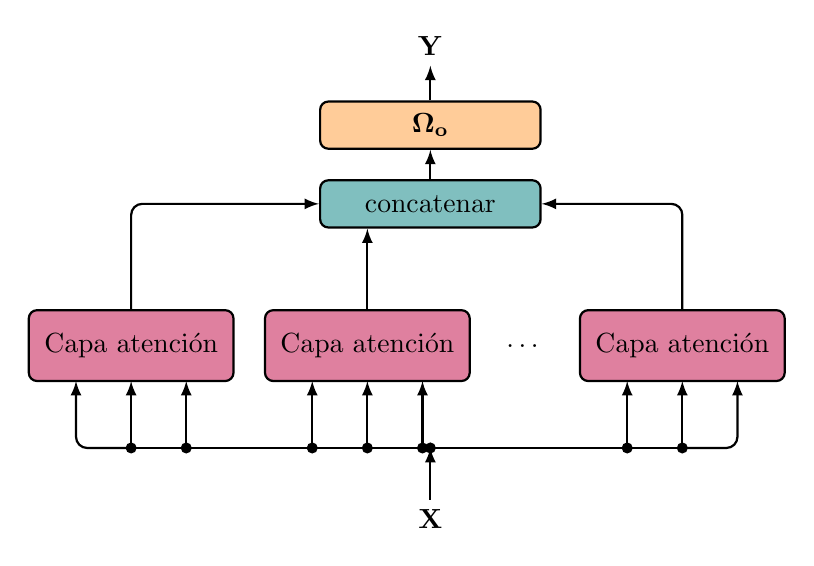
\begin{tikzpicture}[
    >=latex,
    attn/.style={draw, thick, fill=purple!50, rounded corners=3pt, minimum width=2.6cm, minimum height=0.9cm, align=center},
    concat/.style={draw, thick, fill=teal!50, rounded corners=3pt, minimum width=2.8cm, minimum height=0.6cm, align=center},
    linear/.style={draw, thick, fill=orange!40, rounded corners=3pt, minimum width=2.8cm, minimum height=0.6cm, align=center}
    ]

    % Input X
    \node (X) at (0, -0.4) {\textbf{X}};
    \draw [thick, ->] (X.north) -- (0, 0.5);
    
    % Horizontal main base line
    \draw [thick] (-3.8, 0.5) -- (3.2, 0.5);
    
    % Leftmost curved arrow
    \draw [thick, rounded corners=4pt, ->] (-3.8, 0.5) -- (-4.5, 0.5) -- (-4.5, 1.35);
    % Rightmost curved arrow
    \draw [thick, rounded corners=4pt, ->] (3.2, 0.5) -- (3.9, 0.5) -- (3.9, 1.35);
    
    % Straight vertical arrows with dots
    \foreach \x in {-3.8, -3.1, -1.5, -0.8, -0.1, 2.5, 3.2} {
        \fill (\x, 0.5) circle (2pt);
        \draw [thick, ->] (\x, 0.5) -- (\x, 1.35);
    }
    
    % Nodos capa de atencion
    \node[attn] (a1) at (-3.8, 1.8) {Capa atención};
    \fill(0, 0.5) circle (2pt);
    \node[attn] (a2) at (-0.8, 1.8) {Capa atención};
    \node at (1.2, 1.8) {\dots};
    \node[attn] (a3) at (3.2, 1.8) {Capa atención};
    
    % Concat node
    \node[concat] (c) at (0, 3.6) {concatenar};
    
    % Linear node
    \node[linear] (l) at (0, 4.6) {$\mathbf{\Omega_o}$};
    
    % Output Y
    \node (Y) at (0, 5.6) {\textbf{Y}};
    
    % Connections from self-attention to concat
    \draw [thick, ->, rounded corners=4pt] (a1.north) |- (c.west);
    \draw [thick, ->] (a2.north) -- (a2.north |- c.south);
    \draw [thick, ->, rounded corners=4pt] (a3.north) |- (c.east);
    
    % Connection from concat to linear
    \draw [thick, ->] (c.north) -- (l.south);
    
    % Connection from linear to Y
    \draw [thick, ->] (l.north) -- (Y.south);
    
\end{tikzpicture}
}


% =====================================
% FIGURA CONCATENAR MATRICES 
% =====================================

\newcommand{\ConcatenarMatrices}{
    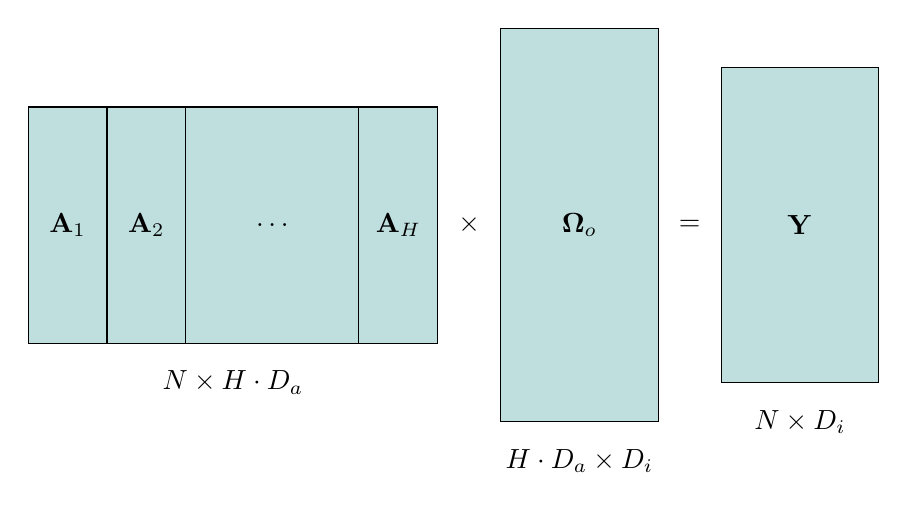
\begin{tikzpicture}

    % Rectángulo grande X
        \fill[teal!50, opacity=0.5] (0,0) rectangle (5.2,3);
        \draw (0,0) rectangle (5.2,3);
        

    %Matriz concatenada
        \draw (0,0) rectangle (1,3);
        \node at (0.5,1.5) {$\mathbf{A}_1$};
        
        \draw (1,0) rectangle (2,3);
        \node at (1.5,1.5) {$\mathbf{A}_2$};
        
        \draw (2,0) rectangle (4.2,3);
        \node at (3.1,1.5) {$\dots$};
        
        
        \node at (4.7,1.5) {$\mathbf{A}_H$};
       
        \node at (2.6,-0.5) {$N \times H \cdot D_a$};

    %Multiplicacion

        \node at (5.6,1.5) {$\times$};

    %Omega output
        \fill[teal!50, opacity=0.5] (6,-1) rectangle (8,4);
        \draw (6,-1) rectangle (8,4);
        \node at (7,1.5) {$\mathbf{\Omega}_o$};

        \node at (7,-1.5) {$H \cdot D_a  \times D_i$};

    %igualdad

        \node at (8.4,1.5) {=};

    %Resultado Y
        \fill[teal!50, opacity=0.5] (8.8,-0.5) rectangle (10.8,3.5);
        \draw (8.8,-0.5) rectangle (10.8,3.5);
        \node at (9.8,1.5) {$\mathbf{Y}$};

        \node at (9.8,-1) {$N \times D_i$};

    \end{tikzpicture}
}


\newcommand{\DiagramaTransformer}{
    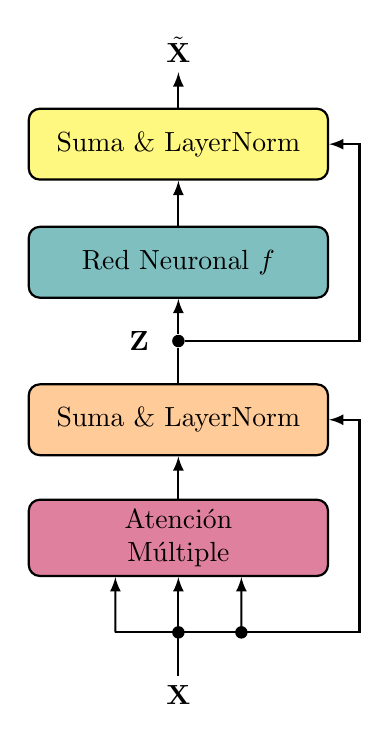
\begin{tikzpicture}[
        >=latex,
        box/.style={
            draw, thick, rounded corners=4pt, 
            minimum width=3.8cm, minimum height=0.9cm, 
            align=center
        },
        attn/.style={box, fill=purple!50},
        addnorm/.style={box, fill=orange!40},
        mlp/.style={box, fill=teal!50},
        dot/.style={circle, fill=black, inner sep=0pt, minimum size=4.5pt},
        final/.style={box, fill=yellow!50}% Puntos de bifurcación
    ]
    
    % 1. Entrada inferior
    \node (x) at (0,0) {$\mathbf{X}$};
    
    % 2. Bloque de Atención
    \node[attn] (mha) at (0, 2) {Atención \\ Múltiple};
    
    % 3. Bifurcaciones y flechas de entrada (Q, K, V)
    \coordinate (c_center) at (0, 0.8);
    \coordinate (c_left) at (-0.8, 0.8);
    \coordinate (c_right) at (0.8, 0.8);
    
    % Líneas horizontales de bifurcación
    \draw[thick] (x) -- (c_center);
    \draw[thick] (c_center) -- (c_left);
    \draw[thick] (c_center) -- (c_right);
    
    % Puntos negros
    \node[dot] at (c_center) {};
    \node[dot] at (c_right) {};
    
    % Flechas hacia el bloque de atención
    \draw[->, thick] (c_center) -- (mha.south);
    \draw[->, thick] (c_left) -- ([xshift=-0.8cm]mha.south);
    \draw[->, thick] (c_right) -- ([xshift=0.8cm]mha.south);


    % 4. Primer bloque Add & Norm
    \node[addnorm] (an1) at (0, 3.5) {Suma \& LayerNorm};
    \draw[->, thick] (mha.north) -- (an1.south);
    
    % 5. Primera conexión residual
    % Parte desde el punto derecho, va hacia la derecha y luego sube
    \draw[->, thick] (c_right) -- (2.3, 0.8) |- (an1.east);
    
    % 6. Variable intermedia z
    \coordinate (z_pos) at (0, 4.5);
    \node[dot] (dot_z) at (z_pos) {};
    \draw[thick] (an1.north) -- (dot_z);
    \node at (-0.5,4.5) {$\mathbf{Z}$};
    
    % 7. Bloque MLP
    \node[mlp] (mlp) at (0, 5.5) {Red Neuronal $f$};
    \draw[->, thick] (dot_z) -- (mlp.south);
    
    % 8. Segundo bloque Add & Norm
    \node[final] (an2) at (0, 7.0) {Suma \& LayerNorm};
    \draw[->, thick] (mlp.north) -- (an2.south);
    
    % 9. Segunda conexión residual
    % Parte desde el punto z, va hacia la derecha y luego sube
    \draw[->, thick] (dot_z) -- (2.3, 4.5) |- (an2.east);
    
    % 10. Salida superior
    \node (xtilde) at (0, 8.2) {$\tilde{\mathbf{X}}$};
    \draw[->, thick] (an2.north) -- (xtilde);
    
    \end{tikzpicture}
}